\section{Data}
\label{sec:data}
%
We have selected the main stock market indices to represent the stock market
performances of MINT and G7 countries. These indices are summarized in 
Table~\ref{tab:variable}: FTSE MIB index for Italy, BIST 100 index for
T\"{u}rkiye, CAC 40 index for France, FTSE 100 index for UK, DAX PERFORMANCE
index for Germany, S\&P 500 index for USA, S\&P/TSX index for Canada, IDX
COMPOSITE index for Indonesia, IPC MEXICO index for Mexico, NIKKEI 225 index for
Japan, and lastly NSE 30 index for Nigeria.  

The data we analyzed was the daily closing prices for the indices collected from
January 30, 2012 to August 14, 2024, accessed from Yahoo
Finance(~\cite{yfinance}) and Investing(~\cite{investing}). 
This date range was selected because the daily values of the Nigerian index NSE
30 is only avalaible from January 30, 2012. Further, the values of the BIST 100
index have been adjusted to reflect the change executed on July 27, 2020. This 
change removed two zeros from the values of the index on that date. Therefore, 
we divided the data preceding this date by 100 to adjust for this change. 

Table~\ref{tab:descriptive} depicts the descriptive statistics of the data. It
can be observed that all indices are non-normal, with the BIST 100 and NSE 30
(stock indices of members of MINT countries) indices being the most positively
skewed and leptokurtic.

Figure~\ref{fig:cor2} summarizes the relationships between the indices according
to the Spearman correlation analysis. Among MINT countries, the least correlated
stock was Nigeria's, followed by Mexico, T\"{u}rkiye, and Indonesia.

Spearman correlation analysis does not take into account the time-dependent 
relationships between the indices. A more appropriate method to analyze the
time-dependent relationships is dynamic time warping (DTW).  DTW is a robust
approach to determine a measure of distance which can be interpreted as a
measure of similarity between two time series, which may vary with time. The
primary concept of DTW is to calculate the distance by comparing corresponding
items in time series that are similar~\citep{dynamic}. Unlike traditional
distance measures, such as Euclidean distance, DTW can handle shifts and
distortions in the time axis and calculates a cumulative distance by considering
the minimum distance path through the cost matrix~\citep{muller2007dynamic}.
Lower DTW distances (close to $0$) indicate that the two time
series are more similar. Figure~\ref{fig:dist2} hence suggests that almost all 
indices show similarity to each other save for the interplay between UK and
Indonesia.

\begin{table*}
    \caption{The variables are the main stock indices of MINT and G7 countries.}
      \label{tab:variable}
      \centering
    \scalebox{0.9}{
\begin{tabular}{@{}ll@{}}
\toprule
\textit{Variable} & \textit{Explanation} \\ \midrule
FTSE MIB   & Price performance of the 40 most-traded stock classes on the Borsa Italiana \\
BIST 100  & Price performance of the 100 largest companies on the Istanbul Stock Exchange \\
CAC 40    & Price performance the 40 most significant stocks on the Euronext Paris\\
FTSE 100   &Price performance of 100 most highly capitalised companies listed on the London Stock Exchange \\
DAX  PERFORMANCE   &Price performance of 30 biggest German companies that trade on the Frankfurt Exchange \\
S\&P 500    & Price performance of 500 of the largest companies listed on stock exchanges in the United States \\
S\&P/TSX    & Stock market index representing roughly 70\% of the total market capitalization on the Toronto Stock Exchange \\
IDX COMPOSITE  & Index of all stocks listed on the Indonesia Stock Exchange \\
IPC MEXICO  &Weighted measurement index of 35 stocks traded on the Borsa Mexico\\
NIKKEI 225   &Stock market index for the Tokyo Stock Exchange\\
NSE 30   &Price performance of 30 companies on the Nigerian Stock Exchange \\ \bottomrule
\end{tabular}
}
\end{table*}

\begin{table*}
    \caption{Descriptive statistics for the main stock indices.}
    \label{tab:descriptive}
    \centering
    \scalebox{0.92}{
\begin{tabular}{@{}llllllllll@{}}
\toprule
\textit{Variable} & \textit{Source} & \textit{Size} & \textit{Mean} & \textit{Median} & \textit{Standard Deviation} & \textit{Minimum} & \textit{Maximum} & \textit{Skewness} & \textit{Kurtosis} \\ \midrule
FTSE MIB     & Yahoo Finance       & 4580       & 21732         & 21494           & 4422.896                    & 12358            & 35401            & 0.713             & 3.590             \\
BIST 100   & Yahoo Finance         & 4580       & 1969        & 977           & 2393.542                    & 541            & 11194          & 2.336             & 7.395             \\
CAC 40       & Yahoo Finance       & 4580       & 5308          & 5139            & 1216.689                    & 2929             & 8242             & 0.423             & 2.417             \\
FTSE 100     & Yahoo Finance       & 4580       & 6914          & 7004            & 644.245                     & 4994             & 8446             & -0.329            & 2.439             \\
DAX         & Yahoo Finance       & 4580       & 11990         & 12101           & 2865.310                     & 5976             & 18875            & 0.112             & 2.475             \\
S\&P 500     & Yahoo Finance       & 4580       & 2886          & 2680            & 1102.271                    & 1278             & 5644             & 0.526             & 2.149             \\
S\&P/TSX         & Yahoo Finance       & 4580       & 16280         & 15582           & 2957.038                    & 11310            & 23105            & 0.439             & 2.098             \\
IDX COMPOSITE        & Yahoo Finance       & 4580       & 5671          & 5779            & 961.285                     & 3697             & 7422             & -0.022            & 1.832             \\
IPC  MEXICO      & Yahoo Finance        & 4580       & 45960         & 45181           & 5118.520                     & 33338            & 58856            & 0.205             & 2.407             \\
NIKKEI 225    & Yahoo Finance      & 4580       & 21605         & 21103           & 7127.358                    & 8279             & 42344            & 0.376             & 2.909             \\
NSE 30      & Investing        & 4580       & 1635          & 1579            & 584.534                     & 872              & 3984             & 2.095             & 8.217             \\ \bottomrule
\end{tabular}
}
\end{table*}

\begin{figure*}
    \centering
    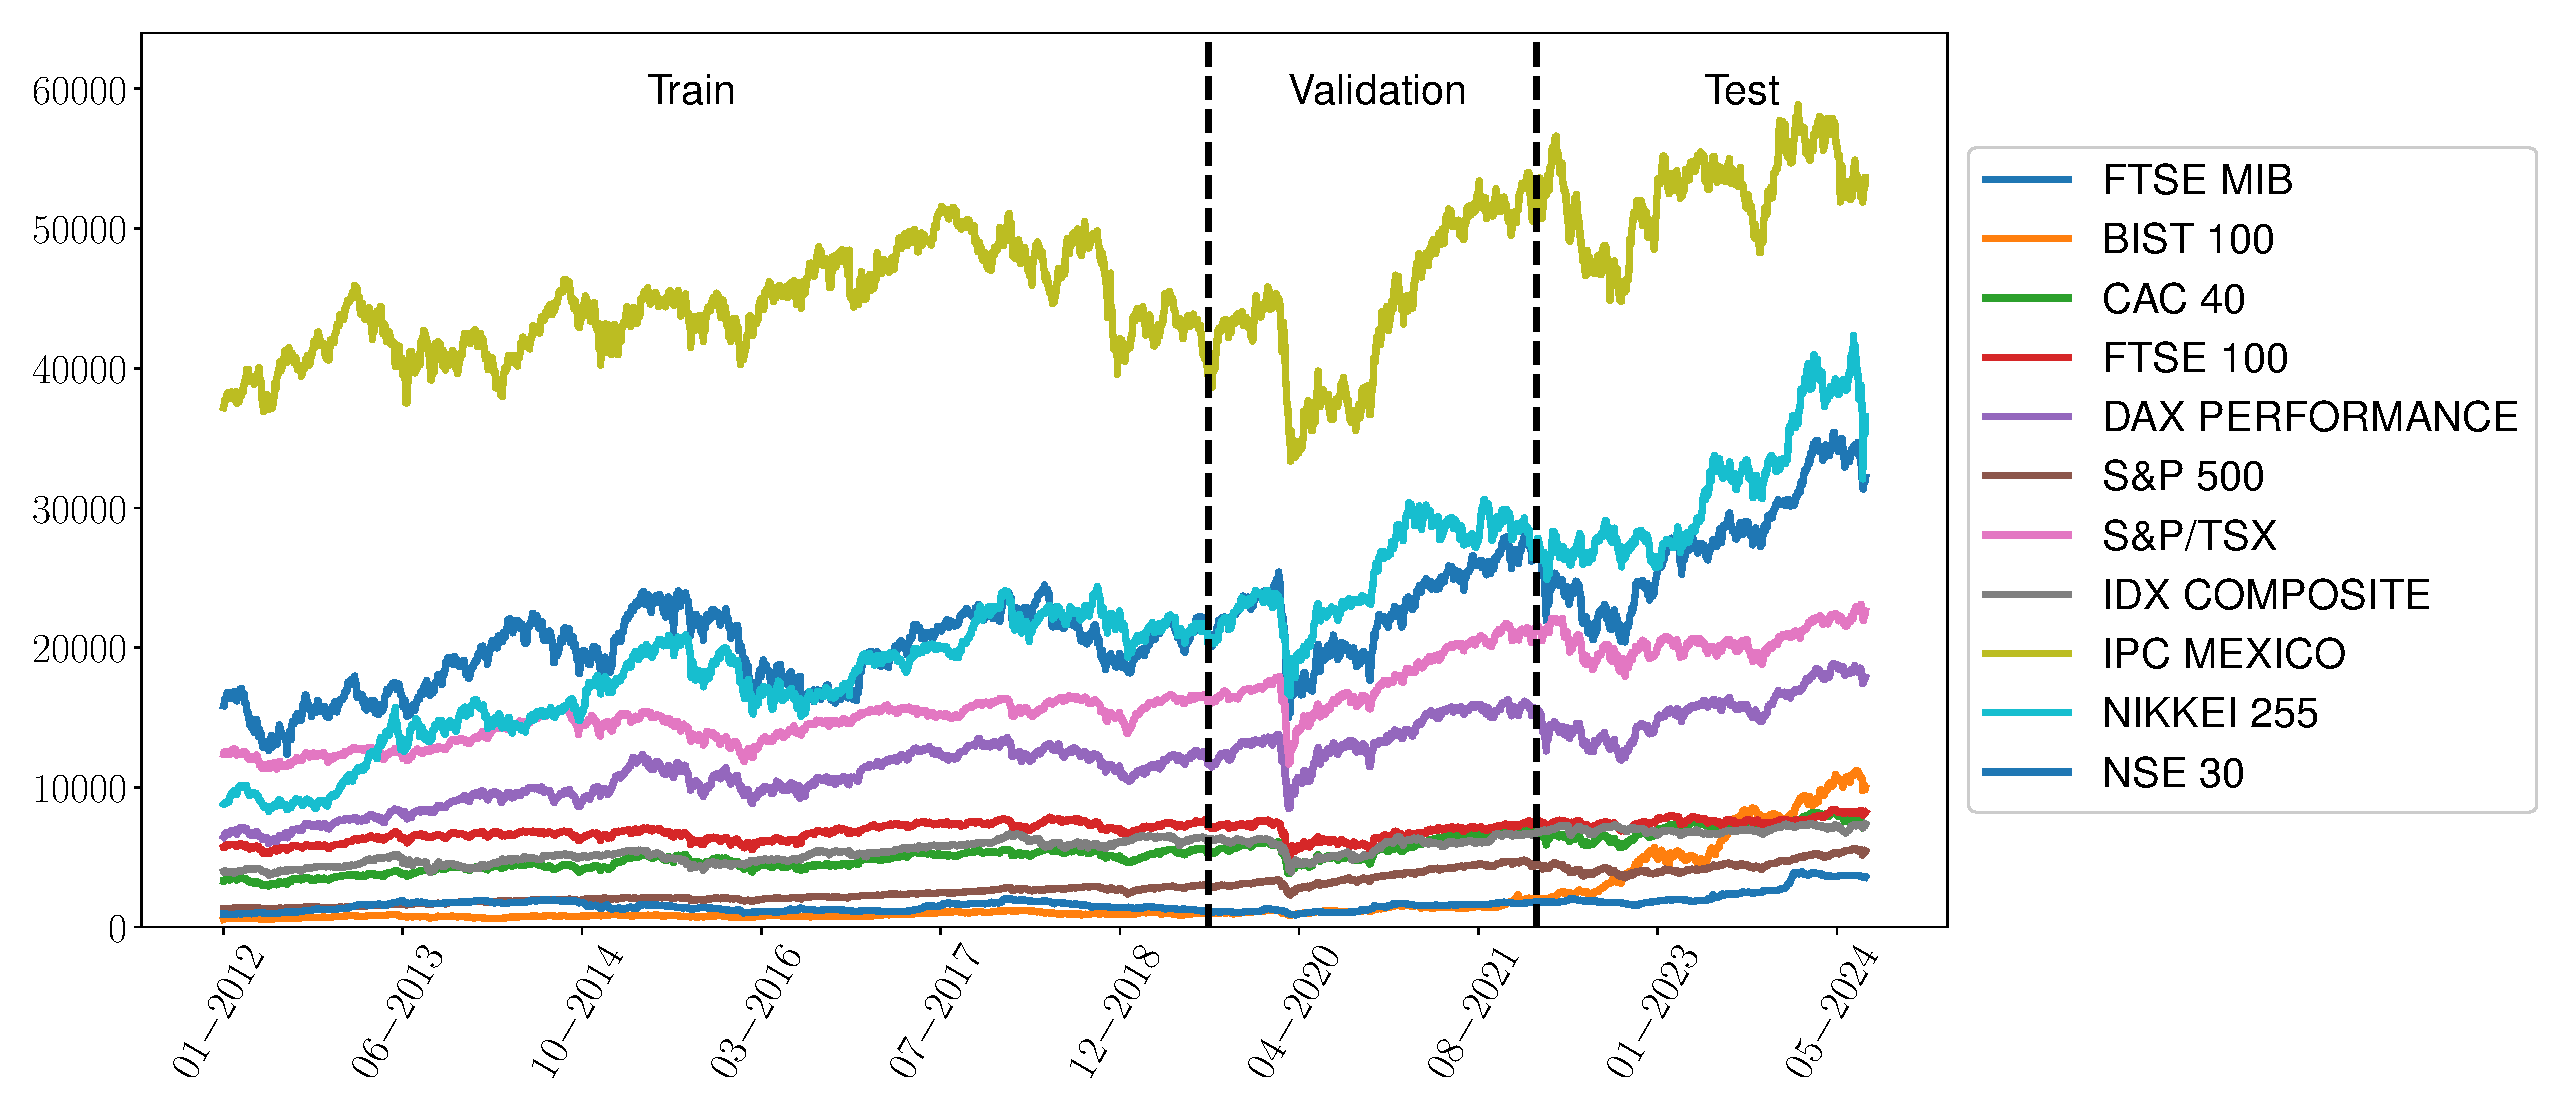
\includegraphics[width=1.0\textwidth]{./figures/alldata.eps}
    \caption{Full glimpse at the processed data: daily closing price of the stock indices.}
    \label{fig:alldata}
\end{figure*}

\begin{figure}[tbh]
  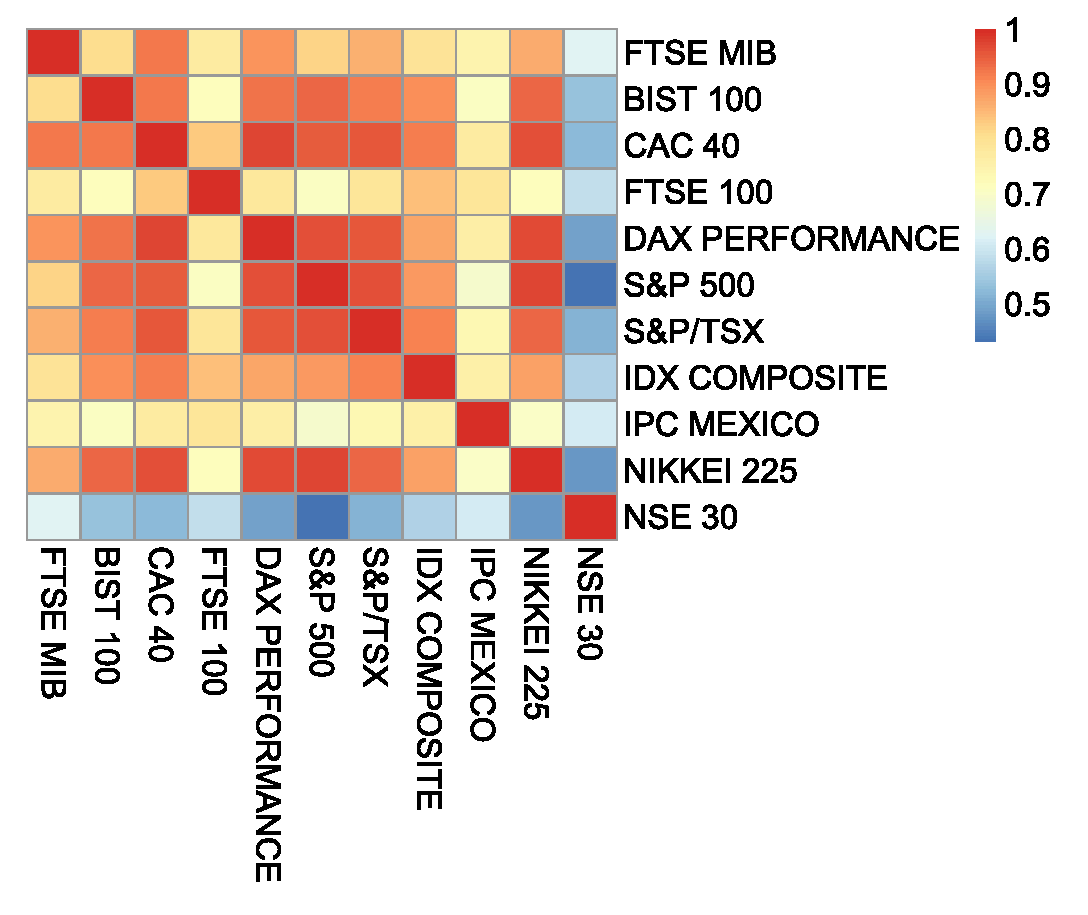
\includegraphics[width=0.47\textwidth]{./figures/cor2.eps}
  \caption{Correlation matrix produced by Spearman correlation analysis.} 
  \label{fig:cor2}
\end{figure}

\begin{figure}[tbh]
  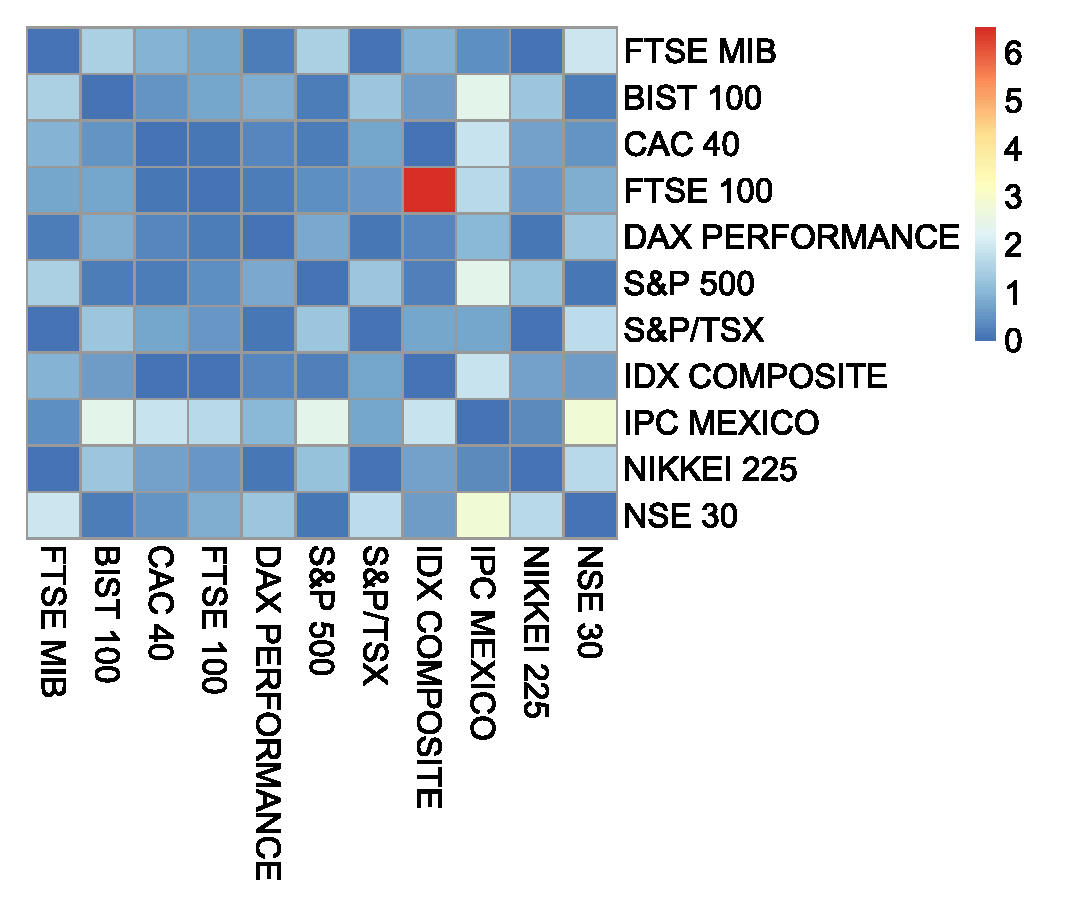
\includegraphics[width=0.47\textwidth]{./figures/dist2.eps}
  \caption{Distance matrix produced by dynamic time warping analysis.} 
  \label{fig:dist2}
\end{figure}

The full data may be observed in Figure~\ref{fig:alldata}. The deep learning 
methods we consider in this work was trained on the initial $60\%$ of the data, 
validated on the next $20\%$, and tested on the final $20\%$ as depicted in this
figure. The data was normalized after getting mapped through a natural logarithm
function to have zero mean and unit variance before training the models.